{\small\textbf{(b)} Matching after the tilt, $x=X$}\par\smallskip
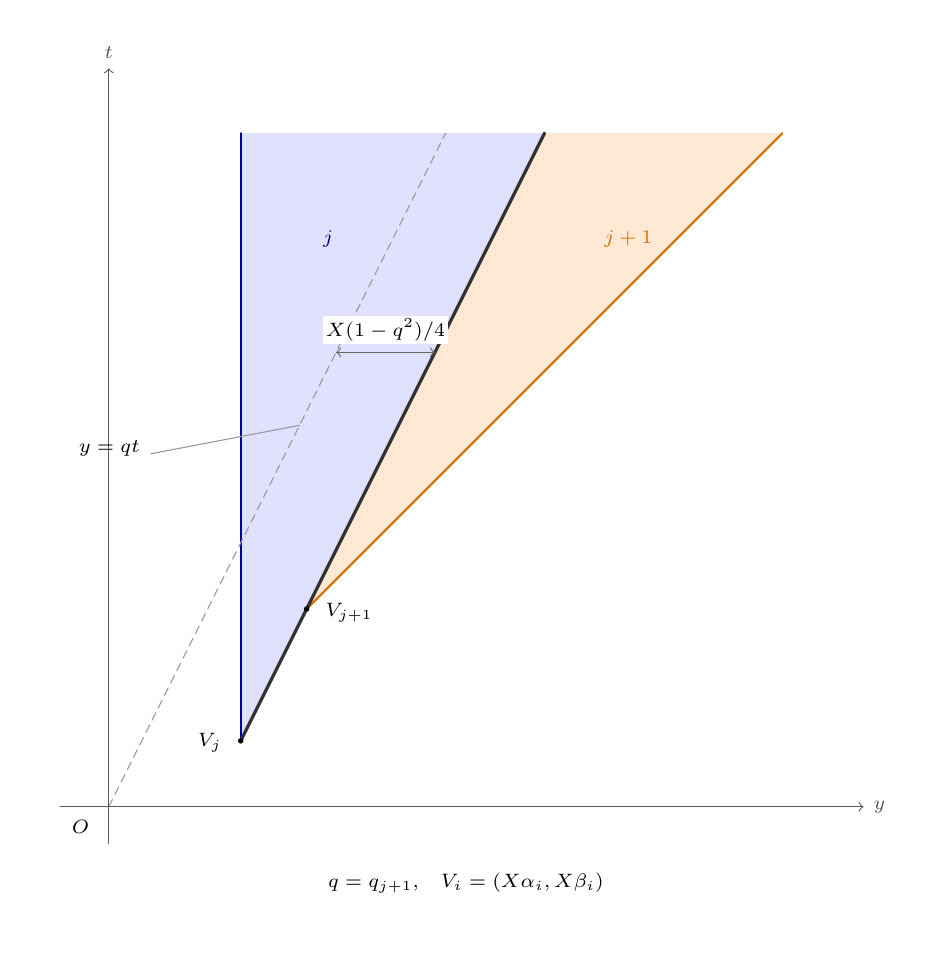
\begin{tikzpicture}[x=0.85\linewidth,y=0.85\linewidth,
  font=\scriptsize,line cap=round,line join=round]
  \coordinate (A) at (.1625,.08125);
  \coordinate (B) at (.24375,.24375);
  \coordinate (Ltop) at (.1625,.83);
  \coordinate (Mtop) at (.536875,.83);
  \coordinate (Rtop) at (.83,.83);
  \fill[blue!12] (A)--(Ltop)--(Mtop)--cycle;
  \fill[orange!17] (B)--(Mtop)--(Rtop)--cycle;
  \draw[blue!65!black,thick] (A)--(Ltop);
  \draw[orange!85!black,thick] (B)--(Rtop);
  \draw[black!80,very thick] (A)--(Mtop);
  \draw[black!40,densely dashed] (0,0)--(.415,.83);
  \draw[<->,black!60] (.28,.56)--(.401875,.56);
  \node[fill=white,inner sep=1pt,anchor=south] at (.3409375,.57)
    {$\eps X(1-q^2)/4$};
  \draw[->,black!65] (-.06,0)--(.93,0) node[right] {$y$};
  \draw[->,black!65] (0,-.045)--(0,.91) node[above] {$t$};
  \node[anchor=north east] at (-.012,-.005) {$O$};
  \fill (A) circle[radius=1pt];
  \fill (B) circle[radius=1pt];
  \node[anchor=east] at (.151,.079) {$V_j$};
  \node[anchor=west] at (.255,.239) {$V_{j+1}$};
  \node[blue!65!black] at (.27,.70) {$j$};
  \node[orange!85!black] at (.64,.70) {$j+1$};
  \node[anchor=south east,align=right] at (.05,.42) {$y=qt$};
  \draw[black!40,thin] (.052,.435)--(.235,.47);
  \node[anchor=north,align=center] at (.44,-.07)
    {$q=q_{j+1}$,\quad $V_i=(\eps X\alpha_i,\eps X\beta_i)$};
  \path[use as bounding box] (-.10,-.15) rectangle (1,.96);
\end{tikzpicture}\par
{\scriptsize The common supporting line is $y=qt+\eps X(1-q^2)/4$.}
